\title{Answer Key for Algebra-Based Physics-1: Mechanics (PHYS135A-01)}
\author{Dr. Jordan Hanson - Whittier College Dept. of Physics and Astronomy}
\date{October 16th, 2017}
\documentclass[10pt]{article}
\usepackage[a4paper, total={18cm, 27cm}]{geometry}
\usepackage{outlines}
\usepackage[sfdefault]{FiraSans}
\usepackage{graphicx}

\begin{document}
\maketitle

\section{Vectors and Newton's Laws}
\begin{enumerate}
\item Let $\vec{F}_{\rm 1} = \frac{3}{4}\hat{i} + 1\hat{j}$ N, and $\vec{F}_{\rm 2} = -1\hat{i} + \frac{3}{4}\hat{j}$ N.  a) Give the magnitude of each force.  b) What is the net force?  c) What is the angle between these two forces? \\ \\
a) $\sqrt{\frac{9}{16} + 1} = \sqrt{\frac{9}{16}+\frac{16}{16}} = \sqrt{\frac{25}{16}} = \frac{5}{4}$.  They have the same magnitude.  b) $\vec{F}_{\rm 1} + \vec{F}_{\rm 2} = -\frac{1}{4}\hat{i} + \frac{7}{4}\hat{j}$ N. c) The dot product is $\vec{F}_{\rm 1} \cdot \vec{F}_{\rm 2} = -\frac{3}{4}+\frac{3}{4} = 0$.  Therefore, the angle between them is 90 degrees.
\item Imagine you are sitting in an airplane that has just lifted off with an acceleration vector 20 degrees with respect to horizontal.  Draw a free-body diagram corresponding to you, showing all forces acting on you.
\begin{figure}[ht]
\centering
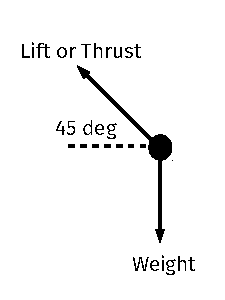
\includegraphics[width=0.2\textwidth]{figures/FBD1.pdf}
\end{figure}
\item Imagine you are riding a skateboard down a hill (no friction), and the incline angle is 30 degrees.  Draw a free-body diagram corresponding to you, showing all forces acting on you.
\begin{figure}[ht]
\centering
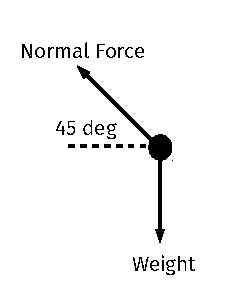
\includegraphics[width=0.2\textwidth]{figures/FBD2.pdf}
\end{figure}
\end{enumerate}
\section{Young's Modulus}
\begin{enumerate}
\item Someone in the laboratory hands us a piece of metal, and needs to know what kind of metal it is.  We decide to measure the Young's modulus, $Y$.  The piece of metal is a cylinder with cross-sectional area $A = 4\pi \times 10^{-4}$ m$^2$, and length $L = 0.1$ m.  We apply a force $F=10^4$ N to squeeze the piece of metal, and the length changes by $x = 10^{-5}$ m.  Young's modulus $Y$ is defined so that:
\begin{equation}
\frac{x}{L} = \frac{p}{Y} = \frac{F/A}{Y}
\end{equation}
What is Y, for this material?  How does this value compare to aluminum or iron? \\
Plugging in the numbers: \\
\begin{equation}
Y = \frac{10^4 N 10^{-1} m}{4\pi 10^{-4} m^2 10^{-5} m} \approx \frac{1}{4\pi} \times 10^{12} Pa \approx 80 \times 10^{9} Pa
\end{equation}
\begin{itemize}
\item $8 \times 10^{8}$ Pa (smaller than most metals by two orders of magnitude)
\item $80 \times 10^{9}$ N (wrong units)
\item $80 \times 10^{9}$ Pa \textbf{(Correct)}
\item $8 \times 10^{9}$ Pa (smaller but close)
\end{itemize}
\end{enumerate}
\section{Frictional Forces}
\begin{enumerate}
\item There is a spill of a mystery toxic liquid on a shop floor, and no one wants to touch it.  Someone gets the bright idea that they can identify it by the coefficient of kinetic friction and a steel plate.  Draw a free body diagram corresponding to a steel plate sliding along the liquid/floor, with friction decelerating it. \\
\begin{figure}[ht]
\centering
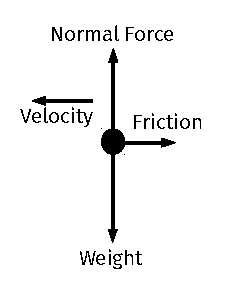
\includegraphics[width=0.2\textwidth]{figures/FBD3.pdf}
\end{figure}
\item What is the coefficient of kinetic friction, $\mu_{\rm k}$, if a steel plate with an initial speed of 2 m/s comes to a stop after 1.0 seconds, assuming $g = 10$ m/s$^2$?  (Use the definition of acceleration $\Delta v/\Delta t = a$). \\ \\
The net force (from the free-body diagram) is $F_{\rm net} = ma = \mu N$.  The normal force is $N = mg$, so we have $ma = \mu m g$, or $a = \mu g$ (acceleration is a fraction of gravity in frictional situations).  But $\Delta v/\Delta t = a$, so $\mu g = \Delta v/\Delta t$, or $\mu = g^{-1} \Delta v/\Delta t$.  Putting in numbers: $\mu = (1/10) 2/1 = 0.2$.
\begin{itemize}
\item 0.1
\item 0.2 \textbf{(Correct)}
\item 0.5
\item 1.2 (Can't be this one, $\mu < 1$)
\end{itemize}
\item Suppose they get a sample of the mystery liquid in a vile.  They assume the drag force is given by Stoke's Law, $F_{\rm D} = 6\pi r \eta v$, where $v$ is the velocity of a particle moving through they fluid, $r$ is the radius of the particle, and $\eta$ is the \textit{viscosity}.  They drop a bead with $r = 1$ mm and a mass of 2 grams into the fluid, and observe the bead sink with a constant (terminal) velocity of 1 m/s.  What is the viscosity of the fluid?  Units: kg/(m s). \\ \\
The corresponding free-body diagram yields: $mg = 6\pi r\eta v$, or $\eta = mg/(6\pi r \eta)$.  Putting in numbers, we have $\eta = 2 10^{-3} 10 / (6\pi 10^{-3} 1) = 10/(3\pi)$.
\begin{itemize}
\item $10/(3\pi)$ kg/(m s) \textbf{(Correct)}
\item $1/(3\pi)$ kg/(m s)
\item $20$ kg/(m s)
\item $10$ kg/(m s)
\end{itemize}
\end{enumerate}
\end{document}